\documentclass[main.tex]{subfiles}
\begin{document}
\chapter{Combinatorics and Probability}

\epigraph{What?!}{Lil Jon}

\minitoc

\section{Introduction}

Combinatorics and probability offer us both a way of thinking and a handful of tools to solve interesting problems. These topics are more real-world focused since they have more direct and obvious applications. The combinatorics mindset can be difficult for some students -- hang in there, you can do it.

This section discusses combinatorics, or \textit{counting arguments}, followed by probability theory and basic statistics. The two topics are related, as you will see later. Probability theory includes discussions on \textit{continuous} probability, however we are exclusively concerned with \textit{discrete} probability (re: the name of this course).

\section{Counting Techniques}

Imagine you are a software developer for a large company, \textit{Macrosoft}. Your manager assigned you to a project that needs testing. Your test cases must cover all execution paths. At first this seems like a daunting task, however you took discrete mathematics and learned about combinatorics. You can calculate exactly how many test cases you need. And so you do -- only to find out that you need \(9! = 362880\) test cases. In the fine words of JonTron, ``that's a lot of damage.''

\begin{defn}[Combinatorics\index{Combinatorics}]
	The area of mathematics dealing with counting
\end{defn}

\exsol{
	Count the number of elements in the following set: \[\{\emptyset, \{a\}, \{b\}, \{a,b\}\}\]
}{
	There are two ways to solve this problem. First, you can visually count the number of elements -- 1, 2, 3, 4. Otherwise, you can notice that the given set is the powerset of \(\{a,b\}\), which is a set of size 2. We know that \(|\mathcal{P}(A)| = 2^{|A|}\), so the number of elements is \(2^2 = 4\).
}

\begin{rem}
	There are almost always multiple valid ways to solve combinatorics problems. Some ways are better than others, though, because they can abstract out to larger inputs.
\end{rem}

\exsol{
	How many different orderings of the letters \textit{abc} can we create?
}{
	We can list all the possible orderings and count them: \textit{abc}, \textit{acb}, \textit{bac}, \textit{bca}, \textit{cab}, \textit{cba}.
	
	Alternatively, we can view this as a 3-letter word where we need to place letters in each of the three positions.
	
	\begin{center}
		\vspace{5mm}
		\rule{1cm}{1pt} \hspace{3mm} \rule{1cm}{1pt} \hspace{3mm} \rule{1cm}{1pt}
		\vspace{5mm}
	\end{center}
	
	For the first position, we have three possibilities: \textit{a}, \textit{b}, or \textit{c}. Then, we place that letter and move on to the second position where we can place one of the two remaining letters. In the last position, we place the remaining letter.
	
	So, \textit{for each} possibility in the first position, we have all possibilities for the second and third positions. So there are \(3 \times \) \textit{second/third position possibilities} total orderings. Then, journey into the second and third positions. There are two remaining letters, so there are \(2 \times \) \textit{third position possibilities} sub-orderings. There is one option in the last position, so putting this all together we get \(3 \times 2 \times 1 = 3! = 6\) total orderings.
	
	\bigskip
	Another way to view this problem is as a decision tree.
	For each step in the tree, we decide which letter to place in the permuted string.
	Then we need to count the number of leaf nodes in the tree.
	\begin{center}
		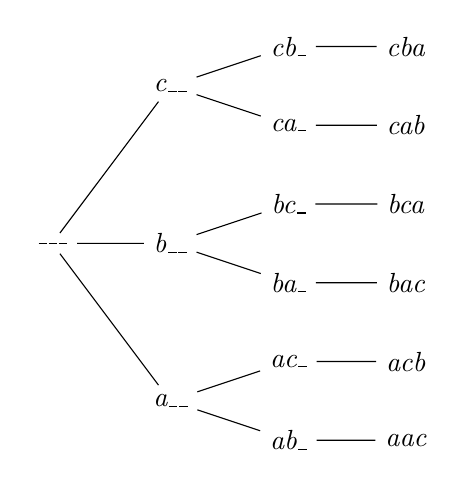
\begin{tikzpicture}[
			level distance=1.5cm,
			level 1/.style={sibling distance=2cm},
			level 2/.style={sibling distance=1cm},
			level 3/.style={sibling distance=1em},
			grow=right
			]
			\node {\textit{\_\_\_}}
			child {node {\textit{a\_\_}}
				child {node {\textit{ab\_}}
					child {node {\textit{aac}}}
				}
				child {node {\textit{ac\_}}
					child {node {\textit{acb}}}
				}
			}
			child {node {\textit{b\_\_}}
				child {node {\textit{ba\_}}
					child {node {\textit{bac}}}
				}
				child {node {\textit{bc\_}}
					child {node {\textit{bca}}}
				}
			}
			child {node {\textit{c\_\_}}
				child {node {\textit{ca\_}}
					child {node {\textit{cab}}}
				}
				child {node {\textit{cb\_}}
					child {node {\textit{cba}}}
				}
			};
		\end{tikzpicture}
	\end{center}
}

%In the example above, we listed out all of the \textit{permutations} of the letters \textit{abc}.

\begin{defn}[Multiplication Rule\index{Combinatorics!Multiplication Rule}]
	Given some procedure \(E\) that can be broken down into a sequence of two tasks, if there are \(n_1\) ways to do the first task and for each of those ways there are \(n_2\) ways to do the second task, then the total number of ways to do procedure \(E\) is \(n_1 \times n_2\)
\end{defn}

\begin{rem}
	This is a highly technical definition that just abstracts the procedure we did the previous example.
\end{rem}

\begin{defn}[Permutations\index{Combinatorics!Permutations}]
	The number of \textbf{ordered} arrangements of \textit{all} elements from a set of size \(n\). By the multiplication rule, the total amount of permutations equals \[n!\]
\end{defn}

\begin{rem}
	\(0! = 1\) -- come back to this later and see if you can make sense of this combinatorially!
\end{rem}

\exsol{
	How many permutations can we make of the string ``rock''?
}{
	By definition, there are \(4! = 24\) permutations. If you do not believe me, list them out! In fact, let's do that right now.
	
	\begin{center}
		\textit{rock}, \textit{rokc}, \textit{rcok}, \textit{rcko}, \textit{rkoc}, \textit{rkco},
		
		\textit{orck}, \textit{orkc}, \textit{ocrk}, \textit{ockr}, \textit{okrc}, \textit{okcr},
		
		\textit{crok}, \textit{crko}, \textit{cork}, \textit{cokr}, \textit{ckro}, \textit{ckor},
		
		\textit{kroc}, \textit{krco}, \textit{korc}, \textit{kocr}, \textit{kcro}, \textit{kcor}
	\end{center}
	
	Feel free to check this against the multiplication rule!
}

\begin{rem}
	In larger examples, we will have analogously large answers. For example, the string ``hardest'' has \(7! = 5040\) permutations. \textit{You do not have time to list out that many permutations}.
\end{rem}

This is not the whole story of permutations. What happens when we have repeat objects in our set (which, would not be a set by definition, but bear with us)?

\exsol{
	How many permutations can we make of the string ``rook''?
}{
	Let's list them out, the same way as we did before with ``rock''.
	
	\begin{center}
		\textit{rook}, \textit{roko}, \textit{rook}, \textit{roko}, \textit{rkoo}, \textit{rkoo},
		
		\textit{orok}, \textit{orko}, \textit{oork}, \textit{ookr}, \textit{okro}, \textit{okor},
		
		\textit{orok}, \textit{orko}, \textit{oork}, \textit{ookr}, \textit{okro}, \textit{okor},
		
		\textit{kroo}, \textit{kroo}, \textit{koro}, \textit{koor}, \textit{koro}, \textit{koor}
	\end{center}
	
	Notice that the first row and last row each contain three, instead of six, unique strings -- half the amount. Further, the second and fourth row are duplicates of each other. Now, we will not count \textit{roko} and \textit{roko} (seen as \textit{ro\textsubscript{1}ko\textsubscript{2}} and \textit{ro\textsubscript{2}ko\textsubscript{1}}) as different strings. So there are \(\frac{4!}{2} = 12\) permutations of ``rook''.
}

\begin{rem}
	Notice that we have two instances of the letter `o'. In the original string, we can order the `o' letters in two ways -- \textit{o\textsubscript{1}} comes first in the string, and \textit{o\textsubscript{2}} second, or \textit{o\textsubscript{2}} comes first and \textit{o\textsubscript{1}} second. This ordering is what we are dividing out, since each of these different orderings of \textit{o\textsubscript{1}} and \textit{o\textsubscript{2}} yields the same string.
\end{rem}

\exsol{
	Now consider the string ``ooopp''. How many permutations can we make of this string?
}{
	Recall the idea of dividing out the number of orderings of each repeated letter. We group those duplicate strings together, and count that as one unique permutation. We have 3 `o' letters, and 2 `p' letters. There are 5 total letters, so we have \(\frac{5!}{3!2!}\) permutations.
	
	Let's examine one uniquely defined permutation, ``opopo''. We know that \textit{op\textsubscript{1}op\textsubscript{2}o} is the same as \textit{op\textsubscript{2}op\textsubscript{1}o}. But now we have three instances of `o'. For each of the previous orderings, we have \textit{o\textsubscript{1}po\textsubscript{2}po\textsubscript{3}}, \textit{o\textsubscript{1}po\textsubscript{3}po\textsubscript{2}}, \textit{o\textsubscript{2}po\textsubscript{1}po\textsubscript{3}}, \textit{o\textsubscript{2}po\textsubscript{3}po\textsubscript{1}}, \textit{o\textsubscript{3}po\textsubscript{1}po\textsubscript{2}}, \textit{o\textsubscript{3}po\textsubscript{2}po\textsubscript{1}}. So by the multiplication rule, we have \(2 \times 6 = 2! \times 3!\) different ``orderings'' of the same word. So for each permutation of ``ooopp'', we can group \(2! \times 3! = 12\) of those permutations into the same string. So we divide out this amount from the entire permutation.
}

\begin{defn}[\(r\)-Permutation\index{Combinatorics!r-Permutations}]
	\textbf{Ordered} arrangements of \(r\) elements from a set of size \(n\). The total amount of \(r\)-permutations is denoted, and equals, \[P(n,r) = \frac{n!}{(n-r)!}\]
\end{defn}

Why does this formula work? Well, use our previous definition of a permutation to permute a set of size \(n\). Then, consider our \(r\) elements as unique letters in a string, and consider the other \(n-r\) elements as the same letter. Then use the previous idea to conclude that there are \(\frac{n!}{(n-r)!}\) permutations.

\begin{rem}
	In the previous paragraph, we gave a \textit{combinatorial argument}.
\end{rem}

\exsol{
	We are a combinatorics photographer. A group of 7 students walked into our office asking for all different possible pictures of them with only 3 people. Since we charge per-photo, how many such photos will we take?
}{
	We \textit{could} count out all of the options, but that might be too much work. Instead, we can translate the problem into a string problem like before. We want all possibilities of 3 people in a row:
	
	\begin{center}
		\vspace{5mm}
		\rule{1cm}{1pt} \hspace{3mm} \rule{1cm}{1pt} \hspace{3mm} \rule{1cm}{1pt}
		\vspace{5mm}
	\end{center}
	
	In the first position, we have 7 possibilities. Then, in the second position, we have 6 possibilities. Finally, in the third position, we have 5 possibilities. Thus, in total, we can make \(7 \times 6 \times 5\) photos.
	
	Alternatively, we could have used \(r\)-permutations. In this case, \(r = 3\) and \(n = 7\). So we are finding all 3-permutations of a set of size 7. This is \[P(7,3) = \frac{7!}{(7-3)!} = \frac{7!}{4!} = 7 \times 6 \times 5\]
}

\begin{defn}[\(r\)-Combinations\index{Combinatorics!Combinations}]
	(or just \textit{Combinations}) \textbf{Unordered} arrangements of \(r\) elements from a set of size \(n\). Alternatively, it is the number of \(r\)-sized subsets of a \(n\)-sized set. The total amount of combinations is denoted and equals \[C(n,r) = \binom{n}{r} = \frac{n!}{r!(n-r)!}\]
\end{defn}

\begin{rem}
	\(\binom{n}{r}\) is often called a \textit{binomial coefficient}.
\end{rem}

\exsol{
	How many student committees of size 3 can we make from a student population of 7?
}{
	There is no notion of \textit{order} within a committee, so we want the number of 3-combinations from a set of size 7. So the answer is \[\binom{7}{3} = \frac{7!}{3!4!}\]
	
	Alternatively, we could first solve the problem as-if we care about the committee ordering, and then \textit{divide out} all of the different possible orderings per committee. For example, the ordered committees \(a,b,c\) and \(b,c,a\) should be counted as the same. So, how many orderings \textit{per-committee} can we make? \(3!\). Then, the total amount of ordered committees is \(P(7,3) = \frac{7!}{4!}\). So if we divide out \(3!\) we get \[\frac{P(7,3)}{3!} = \frac{7!}{3!4!} = \binom{7}{3}\]
}

\begin{rem}
	The previous example shows the relationship between permutations and combinations by showing an easy-to-abstract combinatorial argument.
\end{rem}

There are slight differences between the notion of \textit{with replacement} and \textit{without replacement}. In the former, one would sample a set, record their observation, and put their sample back and keep going. In the latter, one would sample a set, record their observation, \textbf{not} put the sample back, and continue. Keeping this difference in mind will help you tremendously in choosing the correct counting technique to solve a given problem.

\exsol{
	\begin{enumerate}
		\item How many passwords of length 10 can we create if we can only use lowercase English characters?
		
		\item What if we are not allowed to use the same character more than once?
	\end{enumerate}
}{
	In the first problem, we can write out 10 slots with 26 options per slot. The multiplication rule tells us we have \(26^{10}\) possible passwords.
	
	In the second problem, we cannot re-use characters. So we choose the first character (26 options), then choose the second character (25 options -- we cannot use the first chosen character again!), and keep going. This gives us \(26 \times 25 \times \cdots \times 17 = \frac{26!}{(26-10)!}\) possible passwords.
	
	\bigskip
	In the first problem, we are allowed to \textit{re-use} each character -- we sample characters \textit{with replacement}. In the second, we are not -- \textit{without replacement}.
}

\begin{figure}[H]
	\centering
	\begin{tabular}{ccc}
		& With Replacement & Without Replacement \\
		\midrule
		Order Matters & \(n^k\) & \(P(n,k) = \frac{n!}{(n-k)!}\) \\
		\midrule
		Order Does Not Matter & \(\binom{n+k-1}{n-1}\) & \(\binom{n}{k} = \frac{n!}{k!(n-k)!}\) \\
	\end{tabular}
	\caption{Ordering and Replacement -- picking \(k\) elements from \(n\) total elements}
\end{figure}

\begin{rem}
	For explanation on unordered sampling with replacement, \href{https://www.probabilitycourse.com/chapter2/2_1_4_unordered_with_replacement.php}{see here}.
\end{rem}

\exsol{
	How many strings of length 3 can we make using the characters \(\Sigma = \{a,b,c\}\)?
}{
	We are counting elements with replacement where order matters.
	Our main set \(n = 3\) is the number of character choices, and our subset \(k = 3\) is the string length.
	By the table, we can make \(3^3 = 27\) strings.
	
	\bigskip
	Another viable solution to this problem is to use a decision tree, where each branch represents placing one of the three characters in the string.
	\begin{center}
		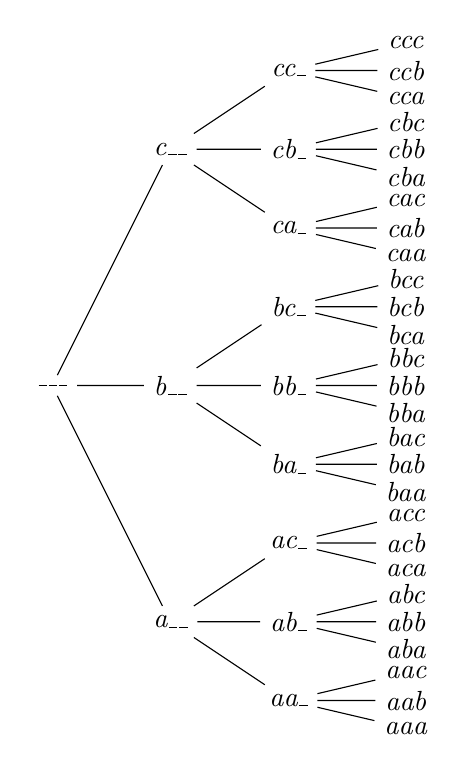
\begin{tikzpicture}[
			level distance=1.5cm,
			level 1/.style={sibling distance=3cm},
			level 2/.style={sibling distance=1cm},
			level 3/.style={sibling distance=1em},
			grow=right
			]
			\node {\textit{\_\_\_}}
			child {node {\textit{a\_\_}}
				child {node {\textit{aa\_}}
					child {node {\textit{aaa}}}
					child {node {\textit{aab}}}
					child {node {\textit{aac}}}
				}
				child {node {\textit{ab\_}}
					child {node {\textit{aba}}}
					child {node {\textit{abb}}}
					child {node {\textit{abc}}}
				}
				child {node {\textit{ac\_}}
					child {node {\textit{aca}}}
					child {node {\textit{acb}}}
					child {node {\textit{acc}}}
				}
			}
			child {node {\textit{b\_\_}}
				child {node {\textit{ba\_}}
					child {node {\textit{baa}}}
					child {node {\textit{bab}}}
					child {node {\textit{bac}}}
				}
				child {node {\textit{bb\_}}
					child {node {\textit{bba}}}
					child {node {\textit{bbb}}}
					child {node {\textit{bbc}}}
				}
				child {node {\textit{bc\_}}
					child {node {\textit{bca}}}
					child {node {\textit{bcb}}}
					child {node {\textit{bcc}}}
				}
			}
			child {node {\textit{c\_\_}}
				child {node {\textit{ca\_}}
					child {node {\textit{caa}}}
					child {node {\textit{cab}}}
					child {node {\textit{cac}}}
				}
				child {node {\textit{cb\_}}
					child {node {\textit{cba}}}
					child {node {\textit{cbb}}}
					child {node {\textit{cbc}}}
				}
				child {node {\textit{cc\_}}
					child {node {\textit{cca}}}
					child {node {\textit{ccb}}}
					child {node {\textit{ccc}}}
				}
			};
		\end{tikzpicture}
	\end{center}
}

\begin{defn}[Combinatorial Argument\index{Combinatorics!Combinatorial Argument}]
	A counting proof that shows a cominatorial identity is true.
	The most common approach is to show two seemingly different quantities \textit{count} the same thing.
\end{defn}

\begin{rem}
	There exist two forms of combinatorial argument.
	\begin{enumerate}
		\item
		Double counting method
		\item
		Bijective method
	\end{enumerate}
	We will focus exclusively on the first.
\end{rem}

One can show that \(X = Y\) via combinatorial argument using the following steps,
\begin{enumerate}
	\item Find/create a counting problem that can be solved in at least two ways
	\item Show that we can count the problem using quantity \(X\)
	\item Show that we can count the problem using quantity \(Y\)
	\item Conclude that, since both ways count same problem, the quantities \(X\) and \(Y\) are equal
\end{enumerate}

\exproof{
	Use a cominatorial argument to show \[2^n = \binom{n}{0} + \binom{n}{1} + \cdots + \binom{n}{n} = \sum_{i=0}^{n} \binom{n}{i}\]
}{
	Consider the problem of counting the number of bit-strings of length \(n\).
	
	We can solve this problem one way by writing out \(n\) slots and for each slot choosing one of two options: \(\{0,1\}\). The multiplication rule tells us this yields \(2^n\) bit-strings.
	
	We can also solve this problem by counting the number of bit-strings that contain zero 1s, one 1, two 1s, three 1s, all the way to \(n\) 1s. This indeed counts all of the bit-strings. There are \(\binom{n}{0}\) bit-strings of length \(n\) with zero 1s. There are \(\binom{n}{1}\) bit-strings of length \(n\) with one 1. Et cetera, there are \(\binom{n}{n}\) bit-strings of length \(n\) with \(n\) 1s. The denominator in each binomial represents the number of slots in the string we are selecting to be a 1. Each of these groups are disjoint, so the total number of bit-strings is their sum: \(\binom{n}{0} + \binom{n}{1} + \cdots + \binom{n}{n}\).
	
	Both counting techniques solve the same problem, so they must be equivalent. Thus \(2^n = \sum_{i=0}^{n} \binom{n}{i}\).
}

\begin{defn}[Algebraic Argument\index{Combinatorics!Algebraic Argument}]
	A proof that argues the correctness of (typically) a combinatorial identity using algebra.
\end{defn}

\exproof{
	Show that \[\binom{n}{k} = \binom{n-1}{k-1} + \binom{n-1}{k}\]
}{
	\begin{align*}
	\binom{n-1}{k-1} + \binom{n-1}{k} &= \frac{(n-1)!}{(k-1)!(n-1-(k-1))!} + \frac{(n-1)!}{k!(n-1-k)!} \\
	&= \frac{(n-1)!}{(k-1)!(n-k)!} + \frac{(n-1)!}{k!(n-k-1)!} \\
	&= \frac{(n-1)!}{(k-1)!(n-k)!}\cdot\frac{k}{k} + \frac{(n-1)!}{k!(n-k-1)!}\cdot\frac{n-k}{n-k} \\
	&= \frac{(n-1)!k + (n-1)!(n-k)}{k!(n-k)!} \\
	&= \frac{(n-1)!(k + (n-k))}{k!(n-k)!} \\
	&= \frac{(n-1)!(n)}{k!(n-k)!} \\
	&= \frac{n!}{k!(n-k)!} = \binom{n}{k}
	\end{align*}
}

The previous example can also be shown using a combinatorial argument.

\exproof{
	Show that \[\binom{n}{k} = \binom{n-1}{k-1} + \binom{n-1}{k}\]
}{
	Consider counting the number of size-\(k\) subsets from a set of size \(n\).
	By definition, there are exactly \(\binom{n}{k}\) subsets.
	On the other hand, we can instead count this quantity by selecting one specific element and counting two disjoint quantities:
	\begin{itemize}
		\item
		picking all size-\(k\) subsets that \textit{include} that element
		\item
		picking all size-\(k\) subsets that \textit{exclude} that element
	\end{itemize}
	For the first, we pick all size-(\(k-1\)) subsets from the remaining \(n-1\) elements and add the specific element into each picked subset.
	We can do this in \(\binom{n-1}{k-1}\) ways.
	For the second, we pick all size-\(k\) subsets from the remaining \(n-1\) elements which all \textit{exclude} the specific element.
	We can do this in \(\binom{n-1}{k}\) ways.
	These are clearly disjoint and cover the entire space, thus we can add their results to yield the total.
}

Usually both argument techniques can show a counting-type identity, however often one technique is better than the other.
As always, unless asked otherwise, it is typically up to you to determine which proof method is better.

\exproof{
	Explain why \(\binom{n}{0} = \binom{n}{n} = 1\).
}{
	We will first show a combinatorial argument, followed by an algebraic argument.
	
	Consider the \textit{meaning} of the binomial coefficient. \(\binom{n}{0}\) means we are choosing 0 elements out of a set of size \(n\). How many ways can we do this? 1 way -- we just pick nothing and leave. Now consider \(\binom{n}{n}\), choosing \(n\) elements out of a set of size \(n\). How many ways can we do this? 1 way -- pull out the entire set (unordered!) and leave. Notice that both outcomes are the same, so they are equal.
	
	Alternatively, consider that \(\binom{n}{0} = \frac{n!}{0!(n-0)!} = \frac{n!}{n!} = 1 = \frac{n!}{n!} = \frac{n!}{n!0!} = \frac{n!}{n!(n-n)!} = \binom{n}{n}\)
}

\begin{thm}[The Binomial Theorem\index{Combinatorics!Binomial Theorem}]
	For \(n \in \N\), \[(x+y)^n = \binom{n}{0}x^n + \binom{n}{1}n^{n-1}y + \binom{n}{2}x^{n-2}y^2 + \cdots + \binom{n}{n-1}xy^{n-1} + \binom{n}{n}y^n\] \[= \sum_{i=0}^{n} \binom{n}{i} x^{n-i}y^i\]
\end{thm}

\begin{proof}
	We offer a quick proof by induction on \(n\). Consider \(n=0\), then \((x+y)^0 = 1\), and \(\sum_{i=0}^{0} \binom{n}{i} x^{n-i}y^i = \binom{0}{0} x^0y^0 = 1\), so they are the same.
	
	Let our hypothesis be for \(n>0\), \((x+y)^{n-1} = \sum_{i=0}^{n-1} \binom{n-1}{i} x^{n-1-i}y^i\).
	
	The step is a bit tricky, so hold on tight. Notice when we use our identity \(\binom{n}{k} = \binom{n-1}{k-1} + \binom{n-1}{k}\).
	\begin{align*}
	\sum_{i=0}^{n} \binom{n}{i} x^{n-i}y^i &= \binom{n}{0} x^n + \sum_{i=1}^{n-1} \binom{n}{i} x^{n-i}y^i + \binom{n}{n} y^n \\
	&= x^n + ( \binom{n}{1}x^{n-1}y + \cdots + \binom{n}{n-1}xy^{n-1} ) + y^n \\
	&= x^n + ( (\binom{n-1}{0} + \binom{n-1}{1})x^{n-1}y + \\
	& \cdots + (\binom{n-1}{n-2} + \binom{n-1}{n-1})xy^{n-1} ) + y^n \\
	&= x^n + ( (\binom{n-1}{0}x^{n-1}y + \binom{n-1}{1}x^{n-1}y) + \\
	& \cdots + (\binom{n-1}{n-2}xy^{n-1} + \binom{n-1}{n-1}xy^{n-1}) ) + y^n \\
	&= x^n + (\sum_{i=0}^{n-2} \binom{n-1}{i} x^{n-1-i}y^{i+1}) \\
	& + (\sum_{i=1}^{n-1} \binom{n-1}{i} x^{n-1-i+1}y^{i}) + y^n \\
	&= x^n + y(\sum_{i=0}^{n-2} \binom{n-1}{i} x^{n-1-i}y^{i}) \\
	& + x(\sum_{i=1}^{n-1} \binom{n-1}{i} x^{n-1-i}y^{i}) + y^n \\
	&\stackrel{\text{IH}}{=} x^n + y((x+y)^{n-1} - \binom{n-1}{n-1}y^{n-1}) \\
	& + x((x+y)^{n-1} - \binom{n-1}{0}x^{n-1}) + y^n \\
	&= x^n + y(x+y)^{n-1} - y^{n} + x(x+y)^{n-1} - x^{n} + y^n \\
	&= y(x+y)^{n-1} + x(x+y)^{n-1} \\
	&= (y+x)(x+y)^{n-1} = (x+y)(x+y)^{n-1} \\
	&= (x+y)^n \\
	\end{align*}
\end{proof}

\begin{rem}
	With this theorem, we can prove that \(2^n = \sum_{i=0}^{n} \binom{n}{i}\). \textit{Hint: set explicit values for \(x\) and \(y\)}.
\end{rem}

\exsol{
	Expand \((x-2)^3\).
}{
	\((x-2)^3 = (x+(-2))^3 = \binom{3}{0}x^3(-2)^0 + \binom{3}{1}x^2(-2)^1 + \binom{3}{2}x^1(-2)^2 + \binom{3}{3}x^0(-2)^3 = x^3 - 6x^2 + 12x - 8\)
}

The Binomial Theorem is helpful in computing the coefficients in a binomial expansion, as seen above. However, remembering the formula may be a hassle. This is where the idea of \textit{Pascal's Triangle} comes into play. We will use the previously-shown identity \(\binom{n}{k} = \binom{n-1}{k-1} + \binom{n-1}{k}\) to help us explain the triangle.

\begin{defn}[Pascal's Triangle\index{Combinatorics!Pascal's Triangle}]
	Construct a discrete triangle of numbers as follows:
	\begin{itemize}
		\item The zero\textsuperscript{th} row is the single number 1
		\item The \(n\)\textsuperscript{th} row consists of \(n\) numbers, where the first and last numbers are a 1, and every in-between number is the sum of the two adjacent numbers in the row above it
	\end{itemize}
\end{defn}

The first 5 rows look like this:
\begin{center}
	\begin{tabular}{ccccccccc}
		&&&& 1 &&&& \\
		&&& 1 && 1 &&& \\
		&& 1 && 2 && 1 && \\
		& 1 && 3 && 3 && 1 & \\
		1 && 4 && 6 && 4 && 1 \\
	\end{tabular}
\end{center}

A keen eye will notice that each number can be expressed as a binomial coefficient dependent on its row and column position:
\begin{center}
	\begin{tabular}{ccccccccc}
		&&&& \(\binom{0}{0}\) &&&& \\
		&&& \(\binom{1}{0}\) && \(\binom{1}{1}\) &&& \\
		&& \(\binom{2}{0}\) && \(\binom{2}{1}\) && \(\binom{2}{2}\) && \\
		& \(\binom{3}{0}\) && \(\binom{3}{1}\) && \(\binom{3}{2}\) && \(\binom{3}{3}\) & \\
		\(\binom{4}{0}\) && \(\binom{4}{1}\) && \(\binom{4}{2}\) && \(\binom{4}{3}\) && \(\binom{4}{4}\) \\
	\end{tabular}
\end{center}

This pattern is explained by our identity \(\binom{n}{k} = \binom{n-1}{k-1} + \binom{n-1}{k}\). Think about what this identity says -- the current binomial coefficient is the sum of two adjacent binomial coefficients in the row above it. To see this, write Pascal's Triangle as a triangular matrix, let the rows be \(n\) and columns be \(k\), and let the first column be \(\binom{n}{0} = 1\) and the diagonal be \(\binom{n}{n} = 1\):
\begin{center}
	\bgroup
	\renewcommand{\arraystretch}{1.5}
	\begin{tabular}{ccccc}
		\(\binom{0}{0}\) & & & & \\
		\(\binom{1}{0}\) & \(\binom{1}{1}\) & & & \\
		\(\binom{2}{0}\) & \(\binom{2}{1}\) & \(\binom{2}{2}\) & & \\
		\(\binom{3}{0}\) & \(\binom{3}{1}\) & \(\binom{3}{2}\) & \(\binom{3}{3}\) & \\
		\(\binom{4}{0}\) & \(\binom{4}{1}\) & \(\binom{4}{2}\) & \(\binom{4}{3}\) & \(\binom{4}{4}\) \\
	\end{tabular}
	\hspace{0.5cm}
	\(=\)
	\hspace{0.5cm}
	\begin{tabular}{ccccc}
		1 & & & & \\
		1 & 1 & & & \\
		1 & 2 & 1 & & \\
		1 & 3 & 3 & 1 & \\
		1 & 4 & 6 & 4 & 1 \\
	\end{tabular}
	\egroup
\end{center}

\begin{thm}[The Multinomial Theorem\index{Combinatorics!Multinomial Theorem}]
	\[(x_1+x_2+\cdots+x_k)^n = \sum_{\substack{i_1, i_2, \cdots, i_k \geq 0 \\ i_1 + i_2 + \cdots + i_k = n}}^{n} \frac{n!}{i_1! i_2! \cdots i_k!} x_1^{i_1} x_2^{i_2} \cdots x_k^{i_k}\]
\end{thm}

We omit the proof on this one, however it is essentially a generalization of the proof for the Binomial Theorem.

\begin{rem}
	You might see \(\frac{n!}{i_1! i_2! \cdots i_k!}\) written as \(\binom{n}{i_1, i_2, \cdots, i_k}\).
	The latter is called the \textit{multi-nomial coefficient}, and is equal to the former.
\end{rem}

\exsol{
	Expand \((x-1+y)^3\).
}{
	Our exponent possibilities are \((0,0,3), (0,3,0), (3,0,0),\\ (1,2,0), (1,0,2), (2,1,0), (0,1,2), (0,2,1), (2,0,1), (1,1,1)\). Thus
	
	\((x-1+y)^3
	= \frac{3!}{0!0!3!}x^0(-1)^0y^3
	+ \frac{3!}{0!3!0!}x^0(-1)^3y^0
	+ \frac{3!}{3!0!0!}x^3(-1)^0y^0
	+ \frac{3!}{1!2!0!}x^1(-1)^2y^0
	+ \frac{3!}{1!0!2!}x^1(-1)^0y^2
	+ \frac{3!}{2!1!0!}x^2(-1)^1y^0
	+ \frac{3!}{0!1!2!}x^0(-1)^1y^2
	+ \frac{3!}{0!2!1!}x^0(-1)^2y^1
	+ \frac{3!}{2!0!1!}x^2(-1)^0y^1
	+ \frac{3!}{1!1!1!}x^1(-1)^1y^1\)
	
	\(= y^3 -1 +x^3 +3x + 3xy^2 -3x^2 -3y^2 + 3y + 3x^2y -6xy\)
}

\exsol{
	Calculate the coefficient of the term \(x^4 y^{1000} z^{200} w^{90}\) in the expansion of \((x-y+2z-2w^3)^{1234}\).
}{
	The coefficient is \(\frac{1234!}{4! 1000! 200! 30!} \cdot 1^4 \cdot (-1)^{1000} \cdot 2^{200} \cdot (-2)^{30}\).
	This follows from the Multinomial Theorem.
	Note that \(w^{90} = (w^3)^{20}\).
	We set \((x_1, x_2, x_3, x_4) = (x, -y, 2z, -2w^3)\) and \((i_1, i_2, i_3, i_4) = (4, 1000, 200, 30)\).
	Then the term in the expansion is
	\(\frac{1234!}{4! 1000! 200! 30!} \cdot x^4 \cdot (-y)^{1000} \cdot (2z)^{200} \cdot (-2w^3)^{30}\).
	By properties of powers, we pull the constant terms \textit{out} and yield
	\(\frac{1234!}{4! 1000! 200! 30!} (1)^4 (-1)^{1000} (2)^{200} (-2)^{30} \cdot x^4 y^{1000} z^{200} w^{90}\).
}

Now, before we move on, we should have a quick discussion as to why \(\binom{n}{k}\) is an integer. It is very tempting to say that, since we can always construct a situation in which \(\binom{n}{k}\) \textit{counts something}, then it is an integer. Indeed, this is a valid \textit{combinatorial argument}. \(\binom{n}{k}\) counts exactly the number of possible \(k\)-subsets from a set of size \(n\). Can we show this a different way? Well, an algebraic argument might not lead anywhere, but an inductive proof may.

% todo : might scrap it?
\exproof{
	Show that \(\binom{n}{k} \in \Z\) for \(n,k \in \N\) and \(n \geq k\).
}{
	First, let us show the following lemma: \[(\forall m \in \N)(\forall o \in \N)[m! \mid \prod_{i=o}^{o+m-1} i]\]
	All this says is that \(m!\) divides the product of \(m\) consecutive integers. We use \(o\) as an \textit{offset}. We will show this with a \textit{double induction} proof on \(m\) and \(o\). Note that \(o\) could be any integer, but we will restrict to naturals for simplicity.
	
	We start by inducting on \(m\). For \(m=0\) then we have \(0! = 1\) and 1 divides everything. So the base case holds.
	
	For a hypothesis, assume \((m-1)! \mid \prod_{i=o}^{o+m-2} i\) for an arbitrary \(m-1 \geq 0\).
	
	For the inductive step, we aim to show \(m! \mid \prod_{i=o}^{o+m-1} i\). We will now show this by inducting on \(o\).
	
	Note that if \(o=0\) then the product is 0, and anything divides 0. We do not have to, but we will also consider \(o=1\). In this case, \(\prod_{i=1}^{1+m-1} i = m!\), and \(m! \mid m!\). So the base case holds.
	
	For a hypothesis, assume \(m! \mid \prod_{i=o-1}^{o-1+m-1} i\) for an arbitrary \(o-1 \geq 0\).
	
	We aim to show that \(m! \mid \prod_{i=o}^{o+m-1} i = (o)(o+1)\cdots(o+m-1)\). Well
	\((o)(o+1)\cdots(o+m-1) = (o-1)(o)\cdots(o-1+m-1) + (o)(o+1)\cdots(o+m-2)\big( (o+m-1) - (o-1) \big) = \prod_{i=o-1}^{o-1+m-1} i + m\prod_{i=o}^{o+m-2} i\). The first term in the sum is divisible by \(m!\) by the induction hypothesis for \(o\). The second term \(\prod_{i=o}^{o+m-2} i\) is divisible by \((m-1)!\) by the induction hypothesis for \(m\). Then \((m-1)! \mid \prod_{i=o}^{o+m-2} i \Rightarrow m(m-1)! \mid m\prod_{i=o}^{o+m-2} i\). Thus our entire original sum is divisible by \(m!\).
	
	So the induction step for \(o\) holds, and thus the induction step for \(m\) also holds.
	
	Then \(\binom{n}{k} = \frac{n!}{k!(n-k)!} = \frac{n \cdot (n-1) \cdots (n-k+1)}{k!}\). Then the numerator is a product of \(n - (n-k+1) + 1 = k-1+1 = k\) consecutive integers, so by the previous lemma \(\binom{n}{k} = \frac{n \cdot (n-1) \cdots (n-k+1)}{k!} \in \Z\).
}

\section{The Inclusion-Exclusion Principle}

Combinatorics deals with counting things. Often we care about counting sizes of sets. Sometimes even when sets overlap, as in a set intersection.
The Inclusion-Exclusion Principle helps us tackle situations when we know \textit{almost} all information about two sets.

\begin{example}
	As a motivating example, let's suppose we wish to count the number of binary strings of length 3 \textit{starting with a 0} \textbf{or} \textit{ending with a 1}.
	A naive approach might be to first calculate the number of strings that start with a 0, and add to that the number of strings that end with a 1.
	
	\begin{multicols}{2}
		Start with 0: 000, 001, 010, 011
		
		\columnbreak
		
		Start with 1: 100, 101, 110, 111
	\end{multicols}
	
	If we do this, then we would yield the solution \(4+4 = 8\).
	Yet, indeed \textit{not all length-3 binary strings start with a 0 or end with a 1}.
	For example, 100 and 110 satisfy neither condition.
	Indeed, the correct answer is \(4+4-2=6\).
	In our naive approach, we forgot to account for the \textit{overlap} between our two cases.
\end{example}

% todo addition rule

% todo subtraction rule

\begin{example}
	Suppose we have 30 students in a class. 10 of them received an A on the first assignment, and 15 of them received an A on the second assignment. 13 students received an A on \textit{both} assignments. How many students have received \textit{at least one} A?
	
	We can visualize this by drawing a Venn-diagram.
	
	\begin{center}
		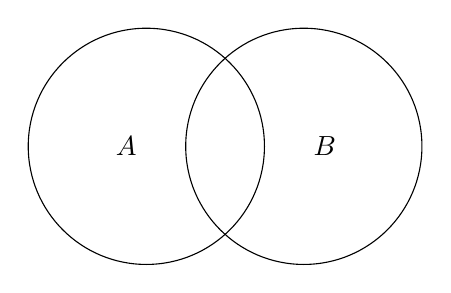
\begin{tikzpicture}
		\draw (0,0) circle (1.5cm) node[left] {\(A\)};
		\draw (0:2cm) circle (1.5cm) node[right] {\(B\)};
		
		\end{tikzpicture}
	\end{center}
	
	We have \(A = \) the students who received an A on the first assignment, and \(B = \) the students who received an A on the second. Then \(|A| = 10\), \(|B| = 15\), and their intersection \(|A \cap B| = 13\). But we are interested in the union -- how can we calculate it?
	
	Well, from the Venn-diagram, we want to find the size of the entire diagram shaded in. How can we use what we know to get \textit{close} to this? Let's try adding \(|A| + |B|\) -- what happens?
	
	\begin{center}
		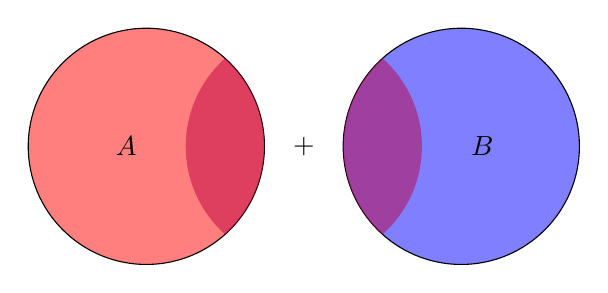
\begin{tikzpicture}
		\fill[red, opacity=0.5] (0,0) circle (1.5cm);
		\draw (0,0) circle (1.5cm) node[left] {\(A\)};
		\draw (0:2cm) node  {\(+\)};
		\fill[blue, opacity=0.5] (0:4cm) circle (1.5cm);
		\draw (0:4cm) circle (1.5cm) node[right] {\(B\)};
		\begin{scope}
			\clip (0,0) circle (1.5cm);
			\fill[purple, opacity=0.5] (0:2cm) circle (1.5cm);
		\end{scope}
		\begin{scope}
			\clip (0:4cm) circle (1.5cm);
			\fill[purple, opacity=0.5] (0:2cm) circle (1.5cm);
		\end{scope}
		\end{tikzpicture}
	\end{center}
	
	Since \(A \cap B \subseteq A\) and \(A \cap B \subseteq B\), then when we add \(|A| + |B|\) we get the entire shaded Venn-diagram \(A \cup B\)! \(\dots\) plus an extra copy of the middle bit \(A \cap B\) \(\dots\).
	
	So just subtract off that extra copy! Then we get \[|A \cup B| = |A| + |B| - |A \cap B|\]
	Now plug in and find that the number of students who received an A is \[10 + 15 - 13 = 12\]
\end{example}

The Inclusion-Exclusion Principle is precisely a generalization of this exact situation. The idea is that we \textit{include} some sets, while we \textit{exclude} some other sets.

\begin{thm}[The Inclusion-Exclusion Principle]
	The size of the union of \(n\) sets equals
	\begin{enumerate}
		\item the inclusion of the sizes of every set
		\item the exclusion of the sizes of every pairwise set intersection
		\item the inclusion of the sizes of every triple-wise set intersection
		\item \textit{and so on}
	\end{enumerate}
	
	More abstractly, for the sets \(A_1,A_2,\cdots,A_n\) we have
	\[|\bigcup_{i=1}^{n} A_i| =\]
	\[\sum_{1 \leq i \leq n} |A_i| - \sum_{1 \leq i,j \leq n} |A_i \cap A_j| + \sum_{1 \leq i,j,k \leq n} |A_i \cap A_j \cap A_k|\]\[- \cdots + (-1)^{n-1}|A_1 \cap \cdots \cap A_n|\]
\end{thm}

\begin{rem}
	The proof of this theorem is essentially the 2-set case but generalized.
\end{rem}

\exsol{
	Calculate the number of students who received \textit{below} an A in all of their first three assignments, given the following information:
	\begin{itemize}
		\item There are 30 students in the class
		\item 8 received an A on assignment 1
		\item 8 received an A on assignment 2
		\item 8 received an A on assignment 3
		\item 6 received an A on assignment 1 and 2
		\item 2 received an A on assignment 1 and 3
		\item 4 received an A on assignment 2 and 3
		\item 1 received an A on all three assignments
	\end{itemize}
}{
	We apply The Inclusion-Exclusion Principle to first calculate the number of people who received an A in any of the first three assignments.
	\begin{align*}
	|A_1 \cup A_2 \cup A_3| &= |A_1| + |A_2| + |A_3| \\
	& - |A_1 \cap A_2| - |A_1  \cap A_3| - |A_2 \cap A_3| \\
	& + |A_1 \cap A_2 \cap A_3| \\
	&= 8+8+8-6-2-4+1 = 13
	\end{align*}
	
	Then the number of people who \textit{did not} get an A is just the total number of students minus those who received an A. \(|(A_1 \cup A_2 \cup A_3)^{c}| = 30 - 13 = 17\)
}

\section{Pigeonhole Principle}

Let us imagine a situation where we have 6 books and 4 bookshelves. Try placing the books on the bookshelves such that each bookshelf only has one book.

\begin{center}
	\textit{Go ahead, I'll wait.}
\end{center}

You can try and try and try, but to no avail. You cannot arrange the books on the shelves such that each shelf contains only one book! Or, equivalently, you know that at least one bookshelf holds more than one book. We formalize this idea as the Pigeonhole Principle -- the books become pigeons and the bookshelves become pigeonholes.

\begin{thm}[The Pigeonhole Principle]
	If \(n\) pigeons are placed into \(k\) pigeonholes, and \(n > k\), then at least one pigeonhole contains more than one pigeon.
\end{thm}

\begin{rem}
	This theorem is somewhat intuitive. Start by placing one pigeon into each hole, then you will have some leftover pigeons. Specifically, you are left with \(n-k\) pigeons. Since \(n > k\) then \(n-k > 0\). So your leftover pigeons have to go somewhere, but all pigeonholes already have a pigeon!
\end{rem}

\begin{proof}
	By contraposition, let all \(k\) containers hold \(\leq 1\) pigeon. Then we add up the total number of pigeons. Denote \(H_i\) to be the number of pigeons in pigeonhole \(i\). The total number of pigeons is \(n = \sum_{i=1}^{k} H_i\). But \(H_i \leq 1\), so \(n = \sum_{i=1}^{k} H_i \leq \sum_{i=1}^{k} 1 = (k-1+1) = k\). So \(n \leq k\).
\end{proof}

\exsol{
	Your birth-month is the month in which you were born. There are 12 birth-months. How many people do we need to gather before we are guaranteed that two of them share a birth-month?
}{
	We use the Pigeonhole Principle. The pigeons are the people we need to gather, and the pigeonholes are the birth-months. Then we need the number of people \(n > 12\). So we need at least 13 people.
}

\begin{thm}[Generalized Pigeonhole Principle]
	If \(n\) objects are placed into \(k\) boxes, then there is at least one box containing at least \(\ceil{\frac{n}{k}}\) objects.
\end{thm}

\begin{proof}
	By contradiction, assume all \(k\) boxes contain \(< \ceil{\frac{n}{k}}\) objects. This is the same as saying that all boxes contain \(\leq \ceil{\frac{n}{k}}-1\) objects. Denote the number of objects in each box \(B_i\). Then the total number of objects is \(n = \sum_{i=1}^{k} B_i \leq \sum_{i=1}^{k} (\ceil{\frac{n}{k}} - 1) = (\ceil{\frac{n}{k}} - 1)(k-1+1) = k(\ceil{\frac{n}{k}} - 1) < k(\frac{n}{k} + 1 - 1) = n\). So \(n < n\), which is a contradiction.
\end{proof}

\begin{rem}
	Suppose you place \(n\) objects into \(k\) boxes one-by-one, wrapping around to the first box once you reach the end. Then if \(n > k\) we must have that the first box contains more than \(\frac{n}{k}\) objects -- all we have done is grouped the objects into \(k\) groups. Then the ceiling \(\ceil{\frac{n}{k}}\) corresponds to that \textit{plus one} as in the original Pigeonhole Principle.
\end{rem}

\exsol{
	Suppose we have a standard deck of cards -- 13 ranks, 4 suits, which yields \(13 \times 4 = 52\) cards. How many cards must we draw to guarantee that our hand contains at least three cards of all the same suit?
}{
	Intuitively, we can try to ``minimize'' the number of like-suit cards we draw. There are four suits, so first pick 4 cards each with a different suit. Then do it again. Then the suit of the next card will already have been chosen twice, which means we will have three cards of the same suit. This is \(2 \times 4 + 1 = 9\) cards.
	
	This is not rigorous though! It might make intuitive sense, but we should apply our proven theorems. In this case, we will use the Generalized Pigeonhole Principle. Let the number of cards we draw be the objects, and the suits be the boxes. Then we need one of our boxes to contain at least 3 objects. So that box contains at least \(\ceil{\frac{n}{4}} = 3\) objects. Then the smallest \(n\) that satisfies this equation is \(n=9\), because \(\ceil{\frac{9}{4}} = \ceil{2.25} = 3\) but \(\ceil{\frac{8}{4}} = \ceil{2} = 2 \neq 3\).
}

\exsol{
	Assume the same deck of cards as before. How many cards must we draw to guarantee that our hand contains cards from all four suits?
}{
	Intuitively, we can try to ``minimize'' the number of suits we draw, until we are forced to draw the final fourth suit. This means we would draw every card from the first three suits, and then the next card we pick must be from the fourth suit. This yields \(13 \times 3 + 1 = 40\) cards.
	
	Formally, as in the Generalized Pigeonhole Principle, let the objects be the number of cards we draw, and the holes be the \textit{ranks}. Then we need one of our boxes to contain at least four objects (each a different suit of that box's rank). So that box contains at least \(\ceil{\frac{n}{13}} = 4\) objects. Then the smallest \(n\) that satisfies this equation is \(n=40\), because \(\ceil{\frac{40}{13}} = \ceil{3.0769\cdots} = 4\) but \(\ceil{\frac{39}{13}} = \ceil{3} = 3 \neq 4\).
}

\section{Discrete Probability}

We have discussed techniques for counting. We can apply this in a statistical sense when we start counting \textit{events}. Often when we discuss probability, we care about some smaller portion, or subset, of the total amount of possible events.

An easy way to introduce probability is by working through a well-known example -- flipping a coin. Assuming the coin is fair, and coin flips are truly random, then we can start to reason about, given any coin flip, whether the coin will land heads-up or tails-up. Later we will see that we do not need these assumptions to reason about which side lands face-up, but we will assume them now for simplicity.

Suppose we flip a fair and truly random coin. We know that there are only two possible outcomes -- the coin lands heads-up, or the coin lands tails-up. Since the coin is truly \textit{random}, we have no way to predict which side will land face-up. Since the coin is \textit{fair}, then both sides are equally likely to land face-up. We refer to this as a 50/50 chance -- a 50\% chance of landing tails, and a 50\% chance of landing heads. Note that \(50\% = 0.5 = \frac{1}{2}\), which is the likelihood that any \textit{one} of our \textit{two} (heads or tails) events occurs.
\begin{center}
	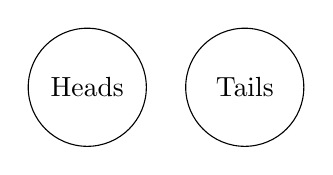
\begin{tikzpicture}
	\draw (0,0) circle (0.75cm) node[] {Heads};
	\draw (2,0) circle (0.75cm) node[] {Tails};
	\end{tikzpicture}
\end{center}

A subtle note on \textbf{percents} -- the \(\%\) symbol. A \textit{percent} is a way to represent \textit{proportions}, or fractions, of a whole. In percent-land, we are concerned with fractions of a single whole, 1. All percents represent numbers in the continuous interval \([0,1]\). To translate a number \(0 \leq r \leq 1\) into a percent, multiply the number by 100 and append a \(\%\) on the end. So \(r \mapsto 100r\%\). For example, \(\frac{1}{4} = 0.25 = 25\%\). Usually percents are approximations for their real-number counterpart -- as such, percents necessarily approximate irrational numbers and any fraction with an infinite decimal expansion. For example, \(\frac{1}{9} = 0.\bar{1} = 0.111111\cdots \approx 11.11\%\). The cutoff point, and whether you round the result, is dependent on the situation -- research \textit{significant figures} if you are interested, but this is irrelevant for this course.

\begin{defn}[Probability\index{Probability}]
	The likelihood (percent chance) that an event occurs.
\end{defn}

\begin{example}
	The probability of flipping tails on a fair 2-sided coin is \(\frac{1}{2}\).
\end{example}

\begin{example}
	The probability of rolling a 2 on a fair 6-sided dice is \(\frac{1}{6}\).
\end{example}

The fractions in a probability are formulated as: \[\frac{\text{\# events wanted}}{\text{\# events possible}}\]
Our previous examples had single events in the numerator, however this fraction lets us extend this to different combinations of events. The numerator and denominator are \textit{counts}, so we can apply any of our previously learned combinatoric methods as well.

\exsol{
	What is the probability of rolling a 2 or a 3 on a 6-sided die?
}{
	We cannot roll a 2 and a 3 at the same time, so we can add their individual probabilities. So the probability is \(\frac{1}{6} + \frac{1}{6} = \frac{1}{3}\).
	
	Alternatively, there are two total different events we care about, out of 6 possible events, so the probability is \(\frac{2}{6}\).
}

\exsol{
	We aim to select a group of size 3, by choosing one-by-one without replacement, from a set of objects \(\{A,B,C,D,E,F,G\}\). What is the probability that our selected group is \(\{A,C,E\}\)?
}{
	Well, how many possible ways can we select exactly those three objects? Note here that the order in which we select the objects does not matter, so long as we end up with \(\{A,C,E\}\). We can translate this to a string problem, selecting letters from \(\{A,C,E\}\) and placing into a length-3 string. This gives us \(3!=6\) possible selections. Then the \(i\)\textsuperscript{th} letter in the string is the \(i\)\textsuperscript{th} object we select. Then how many total possible groups can we select? Well, this is equivalent to asking the amount of possible length-3 strings we can make from our original set, or the amount of 3-permutations. This equals \(P(7,3) = \frac{7!}{4!} = 7 \cdot 6 \cdot 5\). All together, this gives a probability of \(\frac{3!}{\frac{7!}{4!}} = \frac{3!4!}{7!} = \frac{3 \cdot 2 \cdot 1}{7 \cdot 6 \cdot 5} = \frac{1}{35}\).
	
	Alternatively, we could have treated groups as one meaningful package, and examined how many total groups we can make. We can make \(\binom{7}{3}\) groups, one of which is \(\{A,C,E\}\). Then the probability is \(\frac{1}{\binom{7}{3}} = \frac{3!4!}{7!}\) which is the same as before.
}

Now we go back to an earlier example.

\exsol{
	For a 6-sided die, calculate the following probabilities: rolling a 2 or a 3; rolling a 1, 4, or 5; rolling a 6.
}{
	The first set has probability \(\frac{1}{3}\), as we calculated before. The second has probability \(\frac{1+1+1}{6} = \frac{1}{2}\). The third has probability \(\frac{1}{6}\).
}

\begin{rem}
	Notice how \(\frac{1}{3} + \frac{1}{2} + \frac{1}{6} = \frac{2}{6} + \frac{3}{6} + \frac{1}{6} = \frac{2+3+1}{6} = 1\)
\end{rem}

So why does this happen? Well, further notice from the previous example that our three different events are entirely disjoint. Finally, notice that all three events together make up all \textit{possible} events for a 6-sided die. The only possibilities for a 6-sided die is rolling one of the six sides.

Before we formalize this idea, we should establish notation for probabilities.

\begin{defn}[Probability Notation]
	We denote \[P(E) \in [0,1]\] as the probability that event \(E\) occurs.
\end{defn}

\begin{defn}[Sample Space]
	Denote \(\Omega\) as the set of all possible events/outcomes for the current situation.
\end{defn}

\begin{thm}
	Let \(E_1,E_2,\cdots,E_n \in \Omega\). If \(\bigcap_{i=1}^{n} \{E_i\} = \emptyset\) and \(\bigcup_{i=1}^{n} \{E_i\} = \Omega\) then \[\sum_{i=1}^{n} P(E_i) = 1\]
\end{thm}

This intuitively says that the probabilities of disjoint events that cover the entire sample space add to 1. This follows quite easily from the definition of probability -- essentially think of our disjoint sample space as a partition of \([0,1]\), with the lengths of the partition as the probability of the associated event. We saw this happened in the previous example.

\exsol{
	Calculate the probability of \textbf{not} rolling a 1 from a 6-sided die.
}{
	Note that the event \textit{not rolling a 1} is equivalent to rolling a 2 or a 3 or a 4 or a 5 or a 6. Which we can calculate as having probability \(\frac{5}{6}\).
	
	Alternatively, notice how the events \textit{roll a 1} and \textit{not roll a 1} are disjoint. Further notice how these two events entirely make up our sample space of rolling any of the six sides. Then we can apply the previous theorem. Denote the first event as \(E_1\) and the second \(E_2\). We know the probability of rolling a 1, \(P(E_1)\), is \(\frac{1}{6}\). Then we know \(P(E_1) + P(E_2) = 1\), thus \(\frac{1}{6} + P(E_2) = 1\) so \(P(E_2) = 1 - \frac{1}{6} = \frac{5}{6}\).
}

This method, subtracting 1 to find the complement probability, is very common and helpful in more difficult problems. In the previous example, we could easily count all possibilities in the complement event. In other examples, this might not be possible.

\exsol{
	Suppose we roll three 6-sided dice. Our total value from the roll is the sum of all three die. Calculate the probability that our total value is at least 5.
}{
	There are a \textit{lot} of possible rolls that give us a total of at least 5. However, there are significantly less rolls that give us values \textit{strictly less than} 5. We can count them. We have \(\{1,1,1\}\), \(\{2,1,1\}\), \(\{2,2,1\}\), \(\{3,1,1\}\). Then we have a total of \(\frac{6^3}{3!}\) dice rolls (we divide out the \(3!\) possible orderings). So of those dice rolls, we have four that we care about. So \(P(v < 5) = \frac{4}{\frac{6^3}{3!}}\) where \(v\) is the dice roll value. Therefore, \(P(v \geq 5) = 1 - P(v < 5) = 1 - \frac{4}{\frac{6^3}{3!}}\).
}

Now that we understand the idea of joint and disjoint events, we can discuss joint and disjoint \textit{probability}.

\begin{defn}[Joint Probability\index{Probability!Joint}]
	The probability of two (or more) events occurring together. We denote this as \[P(E_1,E_2,\cdots)\]
\end{defn}

We can discuss joint probability for events that are related to each other and for events completely unrelated to each other. This idea of \textit{relation}, that one event may or may not \textit{affect} another, is precisely the idea of \textit{independence}.

\begin{defn}[Independence\index{Probability!Independence}]
	Two events are independent if the outcome of one event does not affect the outcome of the other. More than two events are independent if all possible pairings of events are independent.
\end{defn}

\begin{example}
	The \(n\) events for flipping \(n\) coins are independent.
\end{example}

\begin{example}
	Successive selection events of marbles from a bag, without replacement, are dependent.
\end{example}

\begin{thm}
	If \(E_1\) and \(E_2\) are independent then \(P(E_1 \land E_2) = P(E_1)P(E_2)\)
\end{thm}

\begin{rem}
	You may sometimes see \(P(E_1 \land E_2)\) written as \(P(E_1 \cap E_2)\).
\end{rem}

This is essentially a consequence of our combinatorics multiplication rule.

\exsol{
	Calculate the probability of flipping heads twice in a row. Then calculate the probability of flipping \(n\) heads in a row.
}{
	There is a \(\frac{1}{2}\) probability we flip heads. We know that the second coin flip is independent of the first, so we multiply to get \(\frac{1}{2}\frac{1}{2} = \frac{1}{4}\).
	
	Similarly, for \(n\) flips we get \(\underbrace{\frac{1}{2} \cdot \frac{1}{2}\cdots\frac{1}{2}}_{n \text{ times}} = \frac{1}{2^n}\).
}

Once events start affecting one another, however, then their probabilities act differently.

\exsol{
	Suppose we have a bag of marbles -- 3 red marbles, 2 blue marbles, and 5 green marbles. Calculate the probability of selecting (without replacement) a blue marble, then a red marble, then two green marbles.
}{
	Once we select a marble, notice that the total amount of marbles change. We start with \(3+2+5=10\) marbles. We have 2 blue marbles, so the probability of selecting a blue marble is \(\frac{2}{10}\). Then, we have \(3+1+5=9\) marbles left -- there is one less blue marble. Of these marbles, we have a \(\frac{3}{9}\) probability of selecting a red marble. Then we have \(2+1+5=8\) marbles left. We have a \(\frac{5}{8}\) chance of selecting a green marble. Finally, we have \(2+1+4=7\) marbles left, so we have a \(\frac{4}{7}\) chance of selecting the second green marble.
	
	Now that each probability calculation has accounted for our event dependencies, then we can treat them as independent and multiply to get our resulting probability. This yields \(\frac{2}{10} \cdot \frac{3}{9} \cdot \frac{5}{8} \cdot \frac{4}{7} \approx 2.381\%\).
}

The previous example gives us motivation for a new definition.

\begin{defn}[Conditional Probability\index{Probability!Conditional}]
	The probability of one event occurring given another event occurs. We denote this as \[P(E_2 \mid E_1)\] which reads as \textit{the probability that \(E_2\) occurs given \(E_1\) occurred}.
\end{defn}

\exsol{
	As in the previous example, suppose we have a bag of marbles -- 3 red marbles, 2 blue marbles, and 5 green marbles. Calculate the probability of selecting a red marble \textit{given} we first selected a blue marble.
}{
	Let \(E_1\) represent selecting a blue marble and \(E_2\) represent selecting a red marble. Then \(P(E_2 \mid E_1) = \frac{3}{9}\). In this case, we take out the already-selected blue marble, and continue as usual. There are \(3+1+5=9\) total marbles, and three of those are red.
}

\begin{rem}
	Compare this to the probability of selecting a blue marble and then selecting a red marble (which is \(\frac{2}{10} \cdot \frac{3}{9}\)).
\end{rem}

Think of conditional probability as a re-scale.
In a standard probability, we divide the size of the event by the size of the sample space.
In a \textit{conditional} probability, we change the denominator to the size of the \textit{given} event.
More formally:

\begin{prop}
	\[P(E_2 \mid E_1) = \frac{P(E_2 \cap E_1)}{P(E_1)}\]
\end{prop}

\begin{rem}
	Note that this definition does not work when \(E_1 = \emptyset \Rightarrow P(E_1) = 0\) since we have a divide-by-zero.
	But, note that intuitively \(P(E_2 \mid \emptyset) = P(E_2 \cap \emptyset) = 0\), so it still \textit{somewhat} makes sense.
	The more common  given is
	\[P(E_2 \mid E_1)P(E_1) = P(E_2 \cap E_1)\]
\end{rem}

Now, what if our events in a conditional probability are independent? So what is \(P(E_2 \mid E_1)\) when \(E_1\) and \(E_2\) are independent? Well, the conditional probability focuses on when \(E_2\) occurs \textit{given} \(E_1\) occurred. But \(E_2\) is independent of \(E_1\), so \(E_1\) places no condition on \(E_2\). This gives us our next theorem.

\begin{thm}
	If \(E_1\) and \(E_2\) are independent then \(P(E_2 \mid E_1) = P(E_2)\)
\end{thm}

\exsol{
	Calculate the probability that we flip heads on a coin given we already flipped heads.
}{
	The probability is \(\frac{1}{2}\). In the world where we already flipped heads, well the next flip we do has no dependence on our first flip. So the second flip has the same probability of a standard flip.
}

\exsol{
	What does disjointness tell us about independence?
}{
	For two disjoint events \(E_1\) and \(E_2\) by definition \(E_1 \cap E_2 = \emptyset\).
	Then \(P(E_1 \cap E_2) = \emptyset\).
	For independence to hold, we need \(P(E_1 \mid E_2) = P(E_1)\).
	We know that \(P(E_1 \mid E_2)P(E_2) = P(E_1 \cap E_2)\), so for independence to hold we need
	\[P(E_1)P(E_2) = P(E_1 \cap E_2) = 0\]
	Thus for independence to hold we need one of \(E_1,E_2 = \emptyset\).
	
	This may be counter-intuitive at first -- one may think that disjoint events are indeed independent.
	Yet, while a Venn-diagram interpretation of events gives us information about \textit{conditional} probability, it tells us nothing about \textit{independence}.
	
	The intuition is here -- when two events are mutually exclusive, then either one or the other occurs.
	Thus, if one occurs then the other does not occur (and vice versa).
	This is, in and of itself, a \textbf{dependence} relationship.
}

\begin{defn}[Conditional Independence\index{Probability!Conditional}]
	We say two events \(E_1,E_2\) are independent \textit{given an event \(C\)} if \[P(E_1 \cap E_2 \mid C) = P(E_1 \mid C)P(E_2 \mid C)\]
\end{defn}

\begin{rem}
	This is the same as independence, just given some condition.
\end{rem}

Sometimes a particular conditional probability is difficult to calculate, but the reverse conditional probability is much easier.

\begin{thm}[Bayes' Theorem]
	Let \(P(B) \neq 0\). Then \[P(A \mid B) = \frac{P(B \mid A) \cdot P(A)}{P(B)}\]
\end{thm}

Before we prove this, we need a lemma.

\begin{prop}
	\[P(A \cap B) = P(A)P(B \mid A)\]
\end{prop}

This is simply formalizing our multiplication rule for probabilities, accounting for dependent events.
This is also just a definition of conditional probability.

Then Bayes' holds by getting \(P(A \cap B) = P(A)P(B \mid A)\) and \(P(B \cap A) = P(B)P(A \mid B)\), noticing that \(P(A \cap B) = P(B \cap A)\), and setting these equal \[P(A)P(B \mid A) = P(A \cap B) = P(B)P(A \mid B)\]

\begin{rem}
	Our events in Bayes' theorem are historically written as \(A,B\), but those are simply placeholders. We could have written them as \(E_1,E_2\), \(E,F\), etc.
\end{rem}

\begin{rem}
	There are a few mnemonics to remember this theorem. You can use the proof's formalization, which requires a simple rearrangement to recover the theorem. You can also rearrange the theorem to get \[P(A \mid B) = \frac{P(A) \cdot P(B \mid A)}{P(B)}\] and remember this by remembering \textit{ABABAB}.
\end{rem}

\exsol{
	Bayes' is often used for false positives and false negatives.
	
	Suppose there exists a disease, and a test for this disease.
	Suppose for people who \textit{have} the disease, the test accurately says \textbf{yes} \(90\%\) of the time (true positive).
	Suppose for people who \textit{do not have} the disease, the test falsely says \textbf{yes} \(5\%\) of the time (false positives).
	Suppose finally that \(2\%\) of the world population has this disease.
	You take the test, and it turns up positive.
	What is the probability you actually have the disease?
	Suppose the test turns up negative.
	Do we have enough information to determine if you actually do \textit{not} have the disease?
}{
	We have events \(D\) and \(Y\), representing that you have the \textit{D}isease and representing the test saying \textit{Y}es.
	Our goal is to find \(P(D \mid Y)\) -- the probability you have the disease given the test says you have the disease.
	We know \(P(Y \mid D) = 0.9\) -- the probability that the test says yes given you have the disease.
	We also know \(P(D) = 0.02\) -- the probability that you have the disease, which is just the amount of people in the world who have the disease.
	Then we can use Bayes' so long as we have \(P(Y)\) -- the probability of the test saying yes.
	Well, we know the test says yes in the case that you do have the disease and the case that you do not -- these cover the entirety of our sample space.
	So we can add them.
	\(P(Y \mid D) = 0.9\) and \(P(Y \mid \lnot D) = 0.05\), so \(P(Y) = P(Y \mid D)P(D) + P(Y \mid \lnot D)P(\lnot D) = (0.9)(0.02) + (0.05)(1 - 0.02) = 0.067\).
	Then by Bayes', \(P(D \mid Y) = \frac{P(D)P(Y \mid D)}{P(Y)} = \frac{(0.02)(0.9)}{0.067} \approx 0.2687 \approx 26.87\%\) chance.
	So just above a 1 in 4 chance that you actually have the disease when the test says you do.
	I suppose the test is not very good then.
	
	\bigskip
	
	Now suppose the test says you do not have the disease.
	Then we need the probability that the test says \textit{N}o, \(P(N)\).
	Now, the test either says yes or it says no, and these events are mutually exclusive.
	So \(P(N) = 1 - P(Y) = 1 - 0.067\).
	Then we aim to find \(P(\lnot D \mid N)\), which by Bayes' means we need \(P(\lnot D) = 1 - P(D) = 0.98\) and \(P(N \mid \lnot D)\).
	This is the probability that the test says no given you do not have the disease.
	We know the probability that the test says \textit{yes} given you do not have the disease, \(0.05\).
	Then \(P(N \mid \lnot D) = 1 - P(Y \mid \lnot D) = 1 - 0.05 = 0.95\).
	Indeed we do have enough information!
	Thus by Bayes' \(P(\lnot D \mid N) = \frac{P(\lnot D)P(N \mid \lnot D)}{P(N)} = \frac{(0.98)(0.95)}{1-0.067} \approx 0.9979 \approx 99.79\%\).
	I suppose the test accurately says you do \textit{not} have the disease, so maybe it is not so bad then.
}

\begin{rem}
	The second part of this example reminds us of an interesting idea. \(P(A \mid B) + P(\lnot A \mid B) = 1\).
	However, we know nothing about the relationship between \(P(A \mid B)\) and \(P(A \mid \lnot B)\) (see exercises).
\end{rem}

Note that if events \(A\) and \(B\) are independent then Bayes' tells us that \(P(A) = P(A \mid B) = \frac{P(B \mid A) \cdot P(A)}{P(B)} = \frac{P(B) \cdot P(A)}{P(B)} = P(A)\).
This is not super useful, though.

You may have noticed something in the previous example, where we used an interesting fact about \textit{covering the entire sample space}.
We formalize that here.

\begin{prop}[Marginal Probability]
	For events \(E,A\) we have
	\[P(A) = P(A \mid E)P(E) + P(A \mid \lnot E)P(\lnot E)\]
\end{prop}

\begin{proof}
	\begin{align*}
		   & P(A \mid E)P(E) + P(A \mid \lnot E)P(\lnot E) \\
		=\ & \frac{P(A \cap E)}{P(E)}P(E) + \frac{P(A \cap \lnot E)}{P(\lnot E)}P(\lnot E) \\
		=\ & P(A \cap E) + P(A \cap \lnot E) \\
		=\ & P((A \cap E) \cap (A \cap \lnot E)) + P((A \cap E) \cup (A \cap \lnot E)) \\
		=\ & P(A \cap E \cap \lnot E) + P(A \cap (E \cup \lnot E)) \\
		=\ & P(A \cap \emptyset) + P(A \cap \Omega) \\
		=\ & P(\emptyset) + P(A) = 0 + P(A) = P(A)
	\end{align*}
\end{proof}

\begin{rem}
	This actually abstracts to \(n\) mutually exclusive events that cover the entire sample space (see exercises).
\end{rem}

\section{Basic Statistics\index{Statistics}}

Statistics are an important application of probability. Statistics give us a way to mathematically model probabilities of big events/experiments. We cover three fundamental statistics principles, along with a few related topics.

\begin{rem}
	Before we continue, you may notice that we also write \(\mathrm{Pr}(E)\) to be the probability that event \(E\) occurs. Before, we wrote this as \(P(E)\). These notations are interchangeable.
\end{rem}

\begin{defn}[Random Variable]
	A random variable is an abstraction of a sample space.
\end{defn}

We denote \(X\) as a random variable. Random variables can be discrete or continuous, but we will focus only on the discrete case. Random variables take on values, or outcomes. Typically the outcomes of a random variable are actual values, but can sometimes be events with associated values. All possible random variable outcomes have an associated probability. In the discrete case, we can enumerate each probability. We know that all of these probabilities must add to 1. This also tells us that the probability of an outcome \textit{not} from the random variable has probability 0.

Since the values of \(X\) are numeric values, we can apply our standard mathematical operators. We denote \(\mathrm{Pr}(X = x)\) as the probability that the random variable \(X\) outputs the value \(x\). Similarly, we denote \(\mathrm{Pr}(X > x)\) as the probability that \(X\) is greater than \(x\). We can take the probability of any proposition dependent on \(X\).

\begin{defn}[Expected Value\index{Statistics!Expected Value}]
	\(\mathbb{E}[X] = \mu_X = \sum_{x \in X} x \cdot \mathrm{Pr}(X = x)\). This is a generalization of the \textit{arithmetic mean}, which is defined in scenarios where outcomes are equally likely. If we denote \(x_1, x_2, x_3, \cdots, x_n\) to be the values outputted by \(X\), and \(p_1, p_2, p_3, \cdots, p_n\) to be their respective probabilities, then \(\mathbb{E}[X] = \sum_{i=1}^{n} p_i x_i\)
\end{defn}

Sometimes students confuse \textit{expected value} with \textit{average}. First, the ``average'' is not well-defined -- it could refer to the mean, median, or mode (typically it refers to the mean). Second, as stated in the definition, the expected value is a generalized \textit{mean}. The expected value is precisely the value of the random variable we expect to get.

Note that \[\mathbb{E}[f(X)] = \sum_{x \in X} f(x) \cdot \mathrm{Pr}(X = x)\] which means that the expected value of some function of \(X\) is the same as the expected value of \(X\) but with \(f(x)\) substituted for \(x\).

\begin{prop}
	\(\mathbb{E}\) is a linear function, i.e.\ \(\mathbb{E}[aX+bY] = a\mathbb{E}[X] + b\mathbb{E}[Y]\)
\end{prop}

\begin{proof}
	The expected value of a \textit{value}, not a \textit{variable}, is the value itself: \(\mathbb{E}[v] = v\). If we think of a random variable \(V\) that always outputs \(v\), then  \(\mathrm{Pr}(V=v) = 1\), so \(\mathbb{E}[V] = \sum_{v \in V} v \cdot \mathrm{Pr}(V = v) = v \cdot 1 = v\).
	
	Then the expected value of the sum of variables is the sum of the expected value of those variables: \(\mathbb{E}[X+Y] = \mathbb{E}[X] + \mathbb{E}[Y]\).
	\begin{align*}
	\mathbb{E}[X+Y] &= \sum_{x+y \in X+Y} (x+y) \cdot \mathrm{Pr}(X+Y = x+y) \\
	&= \sum_{x \in X} \sum_{y \in Y} (x+y) \cdot \mathrm{Pr}(X = x \land Y = y) \\
	&= \sum_{x \in X} \sum_{y \in Y} x \cdot \mathrm{Pr}(X = x \land Y = y) \\
	 &+ \sum_{x \in X} \sum_{y \in Y} x \cdot \mathrm{Pr}(X = x \land Y = y) \\
	&= \sum_{x \in X} x \sum_{y \in Y} \mathrm{Pr}(X = x \land Y = y) \\
	 &+ \sum_{y \in Y} y \sum_{x \in X} \mathrm{Pr}(X = x \land Y = y) \\
	&= \sum_{x \in X} x \sum_{y \in Y} \mathrm{Pr}(X = x)\mathrm{Pr}(Y=y \mid X=x) \\
	 &+ \sum_{y \in Y} y \sum_{x \in X} \mathrm{Pr}(Y = y)\mathrm{Pr}(X=x \mid Y=y) \\
	&= \sum_{x \in X} x \cdot \mathrm{Pr}(X = x) \sum_{y \in Y} \mathrm{Pr}(Y=y \mid X=x) \\
	 &+ \sum_{y \in Y} y \cdot \mathrm{Pr}(Y = y) \sum_{x \in X} \mathrm{Pr}(X=x \mid Y=y) \\
	&= \sum_{x \in X} x \cdot \mathrm{Pr}(X = x) + \sum_{y \in Y} y \cdot \mathrm{Pr}(Y = y) \\
	&= \mathbb{E}[X] + \mathbb{E}[Y]
	\end{align*}
	
	These together give us the result.
\end{proof}

\begin{rem}
	Linearity is extended to any countable number of sums and products. So \[\mathbb{E}[c_1 X_1 + c_2 X_2 + \cdots + c_n X_n] = c_1\mathbb{E}[X_1] + c_2\mathbb{E}[X_2] + \cdots + c_n\mathbb{E}[X_n]\]
\end{rem}

\begin{defn}[Variance\index{Statistics!Variance}]
	\(\text{var}(X) = \sigma_X^2 = \mathbb{E}[(X-\mu_X)^2] = \mathbb{E}[(X-\mathbb{E}[X])^2]\)
\end{defn}

\begin{prop}
	\[\sigma_X^2 = \mathbb{E}[X^2] - \mathbb{E}[X]^2\]
\end{prop}

\begin{proof}
	\(\mathbb{E}\) is linear. Then
	\begin{align*}
	\sigma_X^2 &= \mathbb{E}[(X-\mathbb{E}[X])^2] \\
	&= \mathbb{E}[X^2 - 2X\mathbb{E}[X] + \mathbb{E}[X]^2] \\
	&= \mathbb{E}[X^2] - 2\mathbb{E}[X]\mathbb{E}[X] + \mathbb{E}[\mathbb{E}[X]^2] \\
	&= \mathbb{E}[X^2] - 2\mathbb{E}[X]^2 + \mathbb{E}[X]^2 \\
	&= \mathbb{E}[X^2] - \mathbb{E}[X]^2
	\end{align*}
\end{proof}

Variance is a measure for the \textit{spread} of a random variable's sampled output from the variable's expected value.
Variance also leads us to an idea of \textit{Covariance} between two (or more) random variables, which leads us to the idea of random variables being \textit{correlated}. If the covariance between two random variables is zero, then the two random variables are \textit{uncorrelated}, or independent. This is somewhat out of scope for this course, so search online if you are interested.

\begin{defn}[Standard Deviation\index{Statistics!Standard Deviation}]
	\(\text{stdDev}(X) = \sigma_X = \sqrt{\sigma_X^2} = \sqrt{\text{var}(X)}\)
\end{defn}

The standard deviation is also a measure for the spread of a random variable's outcomes from the expected value. In this case, though, the \textit{unit} for standard deviations is the same unit used for the expected value. With variance, however, the unit is the \textit{square} of the expected value's unit. For example, if we had a random variable whose value outputs are in meters, then the expected value's unit will be in meters, the variance's unit will be in meters squared, and the standard deviation's unit will be in meters. Standard deviation is useful for reporting, since its units are easier to understand, but variance is useful for analysis (proofs). The two are entirely dependent on each other, however. With one, you have the other.

Our formulation for the standard deviation is the \textit{population} standard deviation -- when we take a holistic view of the entire output of a random variable. We can also discuss \textit{sample} standard deviation, which estimates the population standard deviation from a random sampling of the random variable. The formula changes, however, since sampling a variable introduces bias in that we could sample the same value more than once. This is a gross oversimplification, however these ideas are out of scope for this course. We encourage you to read more if interested.

We will end with two examples of random variables, and how they give rise to \textit{probability distributions}.

\begin{rem}
	Before we begin, let us introduce some notation. In statistics, the notation \(X \sim Y(\cdot)\) means that \(X\) \textit{is distributed according to} \(Y(\cdot)\). \(Y(\cdot)\) is some function that describes whatever probability distribution you care about.
\end{rem}

\begin{example}
	Suppose \(U_n\) distributes the values \(\{1,2,\cdots,n\}\) each with \textbf{equal} probability. We call \(X \sim U_n\) a \textit{uniform distribution}, since each value is distributed uniformly (equally) as an output. Examples of this include coin flips, dice rolls, picking marbles with replacement, etc.
	
	The expected value of a uniform distribution is \(\mathbb{E}[X] = \sum_{x \in X} x \cdot \mathrm{Pr}(X = x) = \sum_{x=1}^{n} x \cdot \frac{1}{n} = \frac{1}{n}\sum_{x=1}^{n}x = \frac{1}{n}\frac{n(n+1)}{2} = \frac{n+1}{2}\). For example, the expected value of a standard 6-sided die is \(\frac{7}{2} = 3.5\).
	
	\(\mathbb{E}[X]^2 = \frac{1}{n^2}\), so it suffices to calculate \(\mathbb{E}[X^2]\) for the variance. For this, we need to examine \(X^2\), which is the square of each output from \(X\). These values are \(\{1^2,2^2,3^2,\cdots,n^2\}\). The associated probabilities do not change. Then \(\mathbb{E}[X^2] = \sum_{x=1}^{n} x^2 \cdot \frac{1}{n} = \frac{1}{n} \frac{n(n+1)(2n+1)}{6} = \frac{(n+1)(2n+1)}{6}\). Then the variance is
	\(\mathbb{E}[X^2] - \mathbb{E}[X]^2
	= \frac{(n+1)(2n+1)}{6} - (\frac{n+1}{2})^2
	= \frac{(n+1)(2n+1)}{6} - \frac{(n+1)^2}{4}
	= \frac{2(n+1)(2n+1)}{12} - \frac{3(n+1)^2}{12}
	= \frac{2(n+1)(2n+1) - 3(n+1)^2}{12}
	= \frac{(2(2n+1) - 3(n+1))(n+1)}{12}
	= \frac{(n-1)(n+1)}{12}
	= \frac{n^2-1}{12}\).
	For example, the variance of a 6-sided die is \(\frac{6^2-1}{12} = 2.91\bar{6}\).
	
	The standard deviation is the square root of the variance, which in the uniform case is \(\sqrt{\frac{n^2-1}{12}}\). For example, the standard deviation of a 6-sided die is \(\sqrt{2.91\bar{6}} \approx 1.708\).
\end{example}

\begin{rem}
	You thus may see our uniform distribution noted as \(X \sim U(1,n)\), which is abstracted to \(X \sim U(a,b)\) where \(a\) and \(b\), \(a \leq b\), are arbitrary endpoints. In this course, the range between \(a\) and \(b\) is discrete with unit step sizes, however the uniform distribution can be extended to a continuous range.
\end{rem}

\pgfmathdeclarefunction{gauss}{2}{%
	\pgfmathparse{1/(#2*sqrt(2*pi))*exp(-((x-#1)^2)/(2*#2^2))}%
}
\begin{example}
	Suppose \(X\) is a random variable with \(\mu = 0\) and \(\sigma = 1\). We call \(X\) a \textit{standard normal distribution}. It looks like this:
	\medskip
	\begin{center}
		% https://tex.stackexchange.com/a/11371
		\begin{tikzpicture}
		\begin{axis}[every axis plot post/.append
		style={mark=none,domain=-3.5:3.5,samples=50,smooth},
		axis x line=bottom, % no box around the plot, only x and y axis
		axis y line=left, % the * suppresses the arrow tips
		enlarge y limits=upper]
			\addplot {gauss(0,1)};
		\end{axis}
		\end{tikzpicture}
	\end{center}
	
	The x-axis is in units of standard deviations away from the mean, and the y-axis is in percentage of values observed. The area under the graph gives us the total percentage of values observed within a given range. Recall \(\mu=0\) and \(\sigma=1\). We note that \(68.27\%\) of observations are within \(\mu \pm 1\sigma\), \(95.45\%\) within \(\mu \pm 2\sigma\), and \(99.73\%\) within \(\mu \pm 3\sigma\). This tells us that if you sample a normal distribution, there is just above a half chance that your value will be somewhat to the mean, and almost definitely within two standard deviations. We also see that the mean is equal to the median (the midpoint of observations), and is equal to the mode (the most amount of observations) -- look at the tip of the curve! Oh, we also call the normal distribution a \textit{bell curve}, because it kind-of looks like a bell!
	
	We can also \textit{normalize} a random variable. If \(\mu\) and \(\sigma\) are the mean and standard deviation of \(X\) then \(Z = \frac{X - \mu}{\sigma}\) will be roughly normally distributed.
	
	Normal distributions occur in many situations in nature. For example, human height. Another example, student grade data is often normally distributed (this is where the term \textit{curving} comes in, which is when \(\mu\) is low so the ``curve'' is shifted to reduce grade cutoffs). Finally, a \href{https://mathworld.wolfram.com/GaltonBoard.html}{Galton Board}, for large enough trials, approximates a normal distribution.
\end{example}

\section{Summary}

\begin{itemize}
	\item Combinatorics is a toolbox, a mindset, for counting.
	\item Probability often utilizes counting techniques.
	\item Statistics is applied counting and probability.
\end{itemize}

\section{Practice}

\begin{enumerate}
	\item We wish to build a sandwich made of bread, vegetables, cheese, and meat. We can select one of each kind of sandwich substance. There are 8 kinds of breads, 3 kinds of vegetables, 4 kinds of cheese, and 4 kinds of meat. How many possible sandwiches can we make?
	\item In a standard deck of cards, each card has an associated rank (number) \(\in R=\{A,2,3,4,5,6,7,8,9,10,J,Q,K\}\) and suit (symbol) \(\in S=\{\spadesuit,\heartsuit,\diamondsuit,\clubsuit\}\). The set of cards can be abstracted to pairings of ranks and symbols \(C = R \times S\). For example, \((A,\clubsuit)\) is the ace of clubs, and \((7,\spadesuit)\) is the 7 of spades. Typically in card games each player has a \textit{hand}, which is simply a set of cards.
	\begin{enumerate}
		\item Calculate the total amount of \(n\)-card hands. Use this to calculate the total amount of 5-card hands.
		\item A hand has a \textit{pair} if two cards in the hand have the same rank. Calculate the total amount of 5-card hands that have a pair.
		\item There are other types of hands you could have (for example, 3-of-a-kind, straight, full house, etc.). A \textit{straight} is a hand where the cards can be ordered, with wrap-around, in ascending (or descending) order. We let \(A < 2 < \cdots < 10 < J < Q < K\). For example, \(\{(J,\cdot), (Q,\cdot), (K,\cdot), (A,\cdot), (2,\cdot)\}\) is a valid straight. Calculate the total amount of straights. What if we did not allow for wraparound?
		\item A \textit{full house} is a 5-card hand with a pair and a 3-of-a-kind (three cards with the same rank). Calculate the total number of full houses.
		\item Notice that our hands with pairs from (b) include full houses. How many 5-card hands have a pair but are \textbf{not} full houses? Now, these hands also include 3-of-a-kinds and 4-of-a-kinds. Remove these as well. Do we need to remove straights? Do we need to remove 5-of-a-kinds, or any other \(n\)-of-a-kinds?
		\item These have all been related to ranks, but there are also hands related to suits. For example, calculate the total amount of 5-card hands where each card is the same suit. Need these be removed from our set of 5-card hands that are pairs?
	\end{enumerate}
	\item How many ways can you represent \(n \in \Z^+\) as the sum of \(k \in \Z^+\) integers? Solve this by first writing down all cases (as sets) of \(n=5,k=3\). For example, \(\{2,2,1\}\) sum to 5. Then re-write these cases as sums of 1. For example, \(\{1+1,1+1,1\}\). Then find a pattern with the placement of \(,\) (commas) and \(+\) (plus signs) within the 1s.
	\item
	How many terms are in the expansion of \((x_1+x_2+\cdots+x_k)^n\)?
	\item
	How many times does the term \(x_1^{10} x_3^3 x_5^{201}\) appear in the expansion of \((x_1 + x_2 + x_3 + x_4 + x_5)^{214}\)?
	\item
	Calculate the coefficient of the term \(x^4 y^{15} z^{80}\) in the expansion of \((x -2y + 3z^5)^{35}\).
	\item
	Justify why \(0! = 1\) makes sense combinatorially.
	\item
	Show that \(\binom{n}{k} =  \binom{n}{n-k}\) using a cominatorial argument and an algebraic argument.
	\item
	Show that \(P(n,n-1) = P(n,n)\).
	\item Prove that \(\binom{2n}{n} = \sum_{i=0}^{n} \binom{n}{i}^2\).
	\item Prove that \(\binom{n+2}{3} = \sum_{i=1}^{n} i(n-i+1)\).
	\item Prove that \(\binom{m+n}{2} - \binom{m}{2} - \binom{n}{2} = mn\).
	\item Use the Binomial Theorem to show that \(2^0\binom{n}{0} + 2^1\binom{n}{1} + \cdots + 2^n\binom{n}{n} = 3^n\).
	Use this idea to abstract out and show that \(\sum_{i=0}^{n} r^i \binom{n}{i} = (r+1)^n\) for any \(n \in \Z^+\).
	\item
	Show that \(\sum_{k=d}^{n} \binom{n}{k}\binom{k}{d} = 2^{n-d}\binom{n}{d}\).
	\item
	Show that \(\sum_{i=0}^{n-1} \binom{i}{2} = \binom{n}{3}\).
	For this problem, we let \(\binom{i}{2} = 0\) for \(i < 2\).
	\textit{Hint: consider counting size-3 subsets of integers from \(0\) to \(n-1\)}.
	\item
	Show that \(\sum_{i=1}^{n-1} i = \binom{n}{2}\).
	\textit{Hint: come up with a way to enumerate all unique pairings of the integers from 1 to \(n-1\)}.
	\item
	Count the number of binary strings (\(\Sigma = \{0,1\}\)) of length 4 that have the same number of \texttt{0}s than \texttt{1}s.
	What about binary strings of length 5?
	\item
	Count the number of binary strings of length 5 that either start with a \texttt{0} or end with a \texttt{1}.
	\item
	Count the number of ternary strings (\(\Sigma = \{0,1,2\}\)) of length 5 that start with a \texttt{012} or end with a \texttt{10}.
	What about ternary strings of length 4?
	\item
	Suppose we survey 100 computer science students about the programming languages they have used.
	We asked about P \(=\) Python, R \(=\) Ruby, and L \(=\) Lua.
	We yield the following results
	\begin{multicols}{2}
		\begin{itemize}
			\item
			80 students have used P
			\item
			62 students have used R
			\item
			33 students have used L
			\item
			23 students have used P and L
			\item
			25 students have used R and L
			\item
			20 students have used P, R, and L
		\end{itemize}
	\end{multicols}
	Compute the number of students who have used Python and Ruby.
	\item
	Compute the number of \(k\)-intersecting sets that appear in the Inclusion-Exclusion Principle expansion of \(|A_1 \cup A_2 \cup \cdots A_n|\).
	\item
	How many integers between 1 and 10 are divisible by 2? What about 3? What about \textit{both}? What about \textit{neither}?
	Repeat this problem for the range \([1,100] \cap \Z\).
	How many integers in the range \([1,U] \cap \Z\) are divisible by some arbitrary \(n \in \Z^+\)?
	What about some arbitrary range \([L,U] \cap \Z^+\)?
	\item
	What is the smallest prime number \(p^*\) such that every number \(n \in [2,U] \cap \Z\) is divisible by at least one prime \(\leq p^*\), or, formally, find
	\[\underset{p^* \in \P}{\arg\max} \left\{ \big(\forall n \in [2,U] \cap \Z\big) \big(\exists p \in \P^{\leq p^*}\big) \big[p \mid n\big] \right\}\]
	\item
	Suppose you have \(n\) unique \textit{pairs} of socks, where each pair represents two identical socks.
	How many socks must you pull out of your drawer to \textit{guarantee} that you have a matching sock pair?
	\item
	Suppose you have \textit{non-unique} pairs of socks, but the \textit{left} sock is distinguishable from the \textit{right} sock.
	How many socks must you pull out of your drawer to \textit{guarantee} that you have a matching sock pair?
	\item
	Suppose \(n>1\) people shake hands.
	Use the Pigeonhole Principle to justify why there will always be a pair of people that will have performed the same number of handshakes.
	\item
	Suppose \(S = \{1,2,\cdots,9\}\).
	Show that any subset \(A \subseteq S\) with \(|A| = 6\) must contain two elements whose sum is 10.
	Then, let \(S_n = \{1,2,\cdots,n\}\) and compute the minimum number of elements in \(A \subseteq S_n\) required such that at least two elements sum to \(n+1\).
	\item
	How many cards, from a standard 52-deck, must we draw to guarantee we have at least 3 cards from the same suit?
	What about to guarantee we have at least 3 cards from the same rank?
	\item
	Suppose \(M \subseteq \{1,2,\cdots,117\}\) and \(|M| = 10\).
	Do there exist \(A,B \subset M\) such that \(A \cap B = \emptyset\) and \(\sum_{a \in A} a = \sum_{b \in B} b\)?
	\item
	2 of 20 light-bulbs are defective.
	You select two light-bulbs at random. What is the probability that neither bulb selected is defective?
	% (18/20) * (17/19)
	\item
	Suppose a box contains 5 blue marbles, 6 red marbles, and 7 green marbles.
	We pull 3 marbles from the box.
	Compute the probability that our pulled marbles are all different.
	Compute the probability that we pulled at least one blue marble.
	Compute the probability that we pulled one red marble \textit{or} one green marble.
	\item
	Suppose you own a magical ice cream shop that sells two types of ice cream -- the customer's \textit{favorite} flavor, and the customer's \textit{least favorite} flavor.
	Unfortunately, the customer is not allowed to order the ice cream they want, since obviously everyone would just choose their favorite flavor.
	Someone comes in and orders two scoops.
	Scoops are selected, one-by-one (i.e., scoops are independent), with the following probabilities:
	\begin{center}
		\begin{tabular}{ccc}
			& Favorite & Least Favorite \\
			\midrule
			Probability & \(\nicefrac{9}{10}\) & \(\nicefrac{1}{10}\)
		\end{tabular}
	\end{center}
	\begin{enumerate}
		\item
		Let \(F\) be the event that a favorite scoop is selected, and \(L\) be the event that a least favorite is selected.
		You know \(P(F) = \nicefrac{9}{10}\) and \(P(L) = \nicefrac{1}{10}\)
		Calculate the following probabilities:
		\begin{center}
			\begin{tabular}{c|cc}
				& Second scoop \(F\) & Second scoop \(L\) \\
				\hline
				First scoop \(F\) & \(P(FF) =\) & \(P(FL) =\) \\
				First scoop \(L\) & \(P(LF) =\) & \(P(LL) =\) \\
			\end{tabular}
		\end{center}
		\item
		Calculate the conditional probability that the customer receives two of their favorite scoops of ice cream \textit{given} their first scoop is their favorite.
		I.e., calculate \(P(FF \mid F)\).
		\item
		Calculate the conditional probability that they receive two of their favorite scoops of ice cream \textit{given} they have received at least one scoop of their favorite ice cream.
		\item
		Explain what \(P(LL \mid L)\) means, then calculate it.
		\item
		Repeat for \(P(FL \mid L)\).
	\end{enumerate}
	\item
	Suppose \(\Omega\) is a sample space and \(\mathcal{F} = 2^{\Omega}\) is the set of all possible events.
	Show, for mutually exclusive events \(E_1,E_2,\cdots,E_n \in \mathcal{F}\) with \(E_1 \cup E_2 \cup \cdots \cup E_n = \Omega\), for some event \(A \in \mathcal{F}\), that
	\[P(A) = P(A \mid E_1)P(E_1) + P(A \mid E_2)P(E_2) + \cdots + P(A \mid E_n)P(E_n)\]
	\item
	Recall we calculated the probability of flipping \(n\) heads in a row.
	Explain whether this is the same probability as flipping alternating heads and tails.
	Further explain whether the actual pattern of heads and tails matters.
	\item
	Suppose we have a fair coin and a biased coin.
	Each coin can show exclusively either a heads or a tails.
	The fair coin shows heads with probability \(\frac{1}{2}\).
	The biased coin shows heads with probability \(\frac{1}{10}\).
	Suppose we select the fair coin with probability \(\frac{1}{3}\) (and equivalently, the biased coin with probability \(\frac{2}{3}\)).
	After we select the coin, then we solely flip that coin to yield a sequence of heads and tails.
	As an example, \(H^3 T^3 H^2\) would represent flipping 3 heads, followed by 3 tails, followed by 2 heads.
	Note that coin flips are independent.
	Compute \(P(B \mid H^n T^n)\), the probability that we picked the biased coin \textit{given} we flipped \(n\) heads followed by \(n\) tails.
	Then, compute \(\lim\limits_{n \rightarrow \infty} P(B \mid H^n T^n)\).
	Does this make sense?
	Finally, repeat the exercise with \(P(F \mid (HT)^n)\), which is the probability that we roll, \(n\) times, a head followed by a tail (\(HTHTHT \cdots\)).
	
	\item
	Find a relationship between \(P(A \mid B)\) and \(P(A \mid \lnot B)\) \textit{Hint: use Bayes'}.
	
	\item We say that a random variable \(X\) follows a \textit{Bernoulli distribution} if \(X = \{0,1\}\) and \(\mathrm{Pr}(X = 1) = p \in [0,1]\) and \(\mathrm{Pr}(X = 0) = 1-p = q \in [0,1]\). We can describe this as \(X \sim \text{Bernoulli}(p)\) since the Bernoulli is entirely determined by the input probability \(p\). For example, a coin flip is a Bernoulli distribution with \(p=0.5\), \(x=0\) being heads (or tails), and \(x=1\) being tails (or heads). Calculate \(\mu_X\), \(\sigma_X^2\), and \(\sigma_X\).
	
	\item Suppose you are blindly throwing darts at a dart board. You have a \(p \in [0,1]\) chance of actually hitting the target in each independent trial. You wish to model the amount of shots \(k \in \Z^+\) required to successfully hit the target. We say this situation follows a \textit{geometric distribution} with parameter \(p\). Each trial is modeled by a Bernoulli distribution. Let our situation be \(X \sim \text{Geo}(p)\). Then \(\mathrm{Pr}(X = k) = (1-p)^{k-1}p\), which is the probability that you succeed on the \(k\)\textsuperscript{th} trial.
	
	Justify why the probability function above is correct, and calculate the expected trial number of when you successfully hit the target \(\mu_X\). Further, calculate \(\sigma_X^2\) and \(\sigma_X\). Now set \(p=0.25\), a \(25\%\) chance of hitting the target. After how many thrown darts do you expect to hit the target?
\end{enumerate}
\end{document}
